
\documentclass[a4paper,10pt,reqno]{amsart}

\usepackage[T1]{fontenc}

\usepackage{mathdesign}
\usepackage{tgheros}  %  the advanced helvet as it was nice.

\usepackage{siunitx}


% Redefine cite so that we get references in footnotes.
\usepackage[
backend=biber,
citestyle=authoryear,
bibstyle=authoryear,
sorting=none,
firstinits=true
]{biblatex} %style=mla for footnotes.
%\renewcommand{\cite}[1]{\footcite{#1}}
%\renewcommand{\cite}[1]{\supercite{#1}}

\newcommand{\lettr}[1]{#1}

\addbibresource{epilit.bib}
% This has to go below fontenc for some reason
% These lines of code are generated by knitting a .Rtex file.
% We include them here so that we can knit each chapter seperately.
% 

\usepackage{subfig}
\usepackage{color}


%% maxwidth is the original width if it is less than linewidth
%% otherwise use linewidth (to make sure the graphics do not exceed the margin)
\makeatletter
\def\maxwidth{ %
  \ifdim\Gin@nat@width>\linewidth
    \linewidth
  \else
    \Gin@nat@width
  \fi
}
\makeatother

\definecolor{fgcolor}{rgb}{0.345, 0.345, 0.345}
\newcommand{\hlnum}[1]{\textcolor[rgb]{0.686,0.059,0.569}{#1}}%
\newcommand{\hlstr}[1]{\textcolor[rgb]{0.192,0.494,0.8}{#1}}%
\newcommand{\hlcom}[1]{\textcolor[rgb]{0.678,0.584,0.686}{\textit{#1}}}%
\newcommand{\hlopt}[1]{\textcolor[rgb]{0,0,0}{#1}}%
\newcommand{\hlstd}[1]{\textcolor[rgb]{0.345,0.345,0.345}{#1}}%
\newcommand{\hlkwa}[1]{\textcolor[rgb]{0.161,0.373,0.58}{\textbf{#1}}}%
\newcommand{\hlkwb}[1]{\textcolor[rgb]{0.69,0.353,0.396}{#1}}%
\newcommand{\hlkwc}[1]{\textcolor[rgb]{0.333,0.667,0.333}{#1}}%
\newcommand{\hlkwd}[1]{\textcolor[rgb]{0.737,0.353,0.396}{\textbf{#1}}}%

\usepackage{framed}
\makeatletter
\newenvironment{kframe}{%
 \def\at@end@of@kframe{}%
 \ifinner\ifhmode%
  \def\at@end@of@kframe{\end{minipage}}%
  \begin{minipage}{\columnwidth}%
 \fi\fi%
 \def\FrameCommand##1{\hskip\@totalleftmargin \hskip-\fboxsep
 \colorbox{shadecolor}{##1}\hskip-\fboxsep
     % There is no \\@totalrightmargin, so:
     \hskip-\linewidth \hskip-\@totalleftmargin \hskip\columnwidth}%
 \MakeFramed {\advance\hsize-\width
   \@totalleftmargin\z@ \linewidth\hsize
   \@setminipage}}%
 {\par\unskip\endMakeFramed%
 \at@end@of@kframe}
\makeatother

\definecolor{shadecolor}{rgb}{.97, .97, .97}
\definecolor{messagecolor}{rgb}{0, 0, 0}
\definecolor{warningcolor}{rgb}{1, 0, 1}
\definecolor{errorcolor}{rgb}{1, 0, 0}
\newenvironment{knitrout}{}{} % an empty environment to be redefined in TeX

\usepackage{alltt}
\IfFileExists{upquote.sty}{\usepackage{upquote}}{}




\usepackage{caption}
\usepackage{verbatim, geometry, fancyhdr,  graphicx, xcomment, microtype, array}
%\usepackage{amsmath}



\usepackage{bm} % for \bm bold math command for matrices.

\usepackage[pdftex,hidelinks]{hyperref}







\setcounter{tocdepth}{4} % make TOC go to subsubsection



\begin{document}


\title{The role of population structure in pathogen diversity in wild bat populations}
\author{Tim Lucas. \today}
\date{}

\maketitle
%\tableofcontents

\clearpage







\section{Abstract}


\tmpsection{One or two sentences providing a basic introduction to the field}
% comprehensible to a scientist in any discipline.
\lettr{B}ats are an important reservoire of zoonotic diseases.
It is still unclear what factors determine the number of pathogens a wild bat species carries.
But once understood, these factors could provide a way to priorities surveillance of bat populations.


\tmpsection{Two to three sentences of more detailed background}
% comprehensible to scientists in related disciplines.


\tmpsection{One sentence clearly stating the general problem (the gap)}
% being addressed by this particular study.


\tmpsection{One sentence summarising the main result}
%  (with the words “here we show” or their equivalent).


\tmpsection{Two or three sentences explaining what the main result reveals in direct comparison to what was thought to be the case previously}
% or how the main result adds to previous knowledge


\tmpsection{One or two sentences to put the results into a more general context.}



\tmpsection{Two or three sentences to provide a broader perspective, }
% readily comprehensible to a scientist in any discipline.



%%%%%%%%%%%%%%%%%%%%%%%%%%%%%%%%%%%%%%%%%%%%%%%%%%%%%%%%%%%%%%%%%%%%%%%%%%%%%%%%%%%%%%%%%%%%%%%%%%%%%%%%%%%%%%%%%%%%%%%%%%%%%%%%%%%%%%%%%%%%%%%%%%%%%%%%%%%

\clearpage
\section{Introduction}

%%%%%%%%%%%%%%%%%%%%%%%%%%%%%%%%%%%%%%%%%%%%%%%%%%%%%%%%%%%%%%%%%%%%%%%%%%%%%%%%%%%%%%%%%%%%%%%%%%%%%%%%%%%%%%%%%%%%%%%%%%%%%%%%%%%%%%%%%%%%%%%%%%%%%%%%%%%





%%%%%%%%%%%%%%%%%%%%%%%%%%%%%%%%%%%%%%%%%%%%%%%%%%%%%%%%%%%%%%%%%%%%%%%%%%%%%%%%%%%%%%%%%%%%%%%%%%%%%%%%%%%%%%%%%%%%%%%%%%%%%%%%%%%%%%%%%%%%%%%%%%%%%%%%%%%

%\clearpage
\section{Methods}

%%%%%%%%%%%%%%%%%%%%%%%%%%%%%%%%%%%%%%%%%%%%%%%%%%%%%%%%%%%%%%%%%%%%%%%%%%%%%%%%%%%%%%%%%%%%%%%%%%%%%%%%%%%%%%%%%%%%%%%%%%%%%%%%%%%%%%%%%%%%%%%%%%%%%%%%%%%

























































To measure pathogen richness I used data from \cite{luis2013comparison}. 
These simply include known infections of a bat species with a pathogen species. 
Only species with at least one pathogen were included in the analysis.
Rows with host species that were not identified to species level were removed.
Many viruses were not identified to species level or their identified species was not in the ICTV virus taxonomy \cite{ICTV}.
I counted a virus if it was the only virus, for that host species, in the lowest taxonomic level identified in the ICTV taxonomy.
That is, if a host carries an unknown Paramyxoviridae virus, then it must carry at least one Paramyxoviridae virus.
If a host carries an unknown Paramyxoviridae virus and a known Paramyxoviridae virus, then it is hard to confirm that the unknown virus is not another record of the known virus.
In this case, this would be counted as one virus species.






\begin{knitrout}\footnotesize
\definecolor{shadecolor}{rgb}{0.969, 0.969, 0.969}\color{fgcolor}\begin{figure}[t]

{\centering 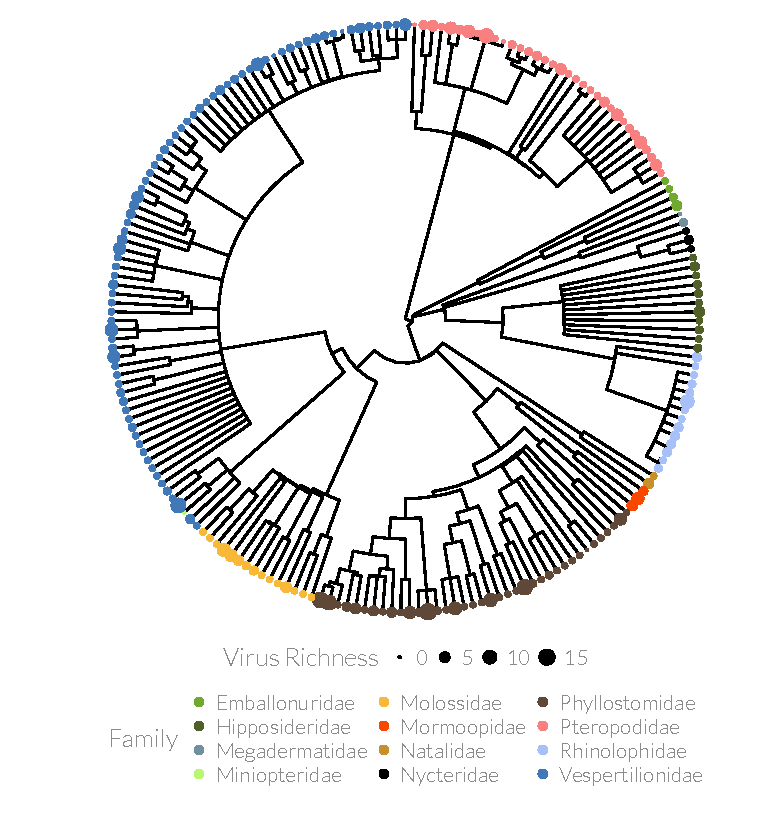
\includegraphics[width=\textwidth]{figure/treePlot-1} 

}

\caption[Pruned phylogeny with dot size showing number of pathogens and colour showing family]{Pruned phylogeny with dot size showing number of pathogens and colour showing family.}\label{fig:treePlot}
\end{figure}


\end{knitrout}












I used two measures of population structure. 
$F_{ST}$ and the number of subspecies.
The number of subspecies was counted using the Wilson and Reeder taxonomy \cite{wilson2005mammal}.
$F_{ST}$ and other measures were collated from the literature.
Studies are from a wide range of spatial scales, from local ($\sim\SI{10}{\kilo\metre}$) to continental.
As $F_{ST}$ inevitably increases with spatial scale I controlled for this by only using data from studies where a large proportion of the species range was studied.
I used the ratio of the furthest distance between $F_{ST}$ samples to the width of the species range and only used studies if this ratio was greater than 0.3.
To allow comparison between different measures ($F_{ST}, \phi_{ST}$) and data from different molecular regions I converted all data to diploid gene flow.
WILL ADD EXTRA METHODS LATER.
These two measures of population structure were analysed separately as the number of subspecies has 196 data points while there is only $F_{ST}$ data for $\sim 30$ bat species.

To control for study bias I collected the number of Pubmed and Google Scholar citations for each bat species including synonyms from ITIS \cite{itis} via the taxize package \cite{chamberlain2013taxize}.
The counts were scraped using the rvest package \cite{rvest}.
I log transformed these variables as they were strongly right skewed.
The log number of citations on Pubmed and Google scholar were highly correlated (pgls: $t$ = 19.32, df = 194, $p$ = 0).
The results here are for analyses using only Google Scholar citations.
See the appendix for analyses run using Pubmed citations.

Measures of body mass are taken from Pantheria \cite{jones2009pantheria} and primary literature \cite{canals2005relative, arita1993rarity, lopez2014echolocation, orr2013does, , lim2001bat, aldridge1987turning, ma2003dietary, owen2003home, henderson2008movements, heaney2012nyctalus, oleksy2015high, zhang2009recent}. 
\emph{Pipistrellus pygmaeus} was assigned the same mass as \emph{P. pipistrellus} as they indistinguishable by mass.
Body mass measurements were log transformed due to the strong right skew.
Distribution size was estimated by downloading range maps for all species from IUCN \cite{} and were also logged due to right skew.

%Pubmed was scraped on pubmedScrapeDate and Google Scholar was scraped on scholarScrapeDate

To control for phylogenetic nonindependance I used the best-supported phylogeny from \cite{fritz2009geographical} which is the supertree from \cite{bininda2007delayed} with names updated to match the Wilson \& Reeder taxonomy \cite{wilson2005mammal}.
Phylogenetic manipulation was performed using the ape package \cite{ape}.
The importance of the phylogeny on each variable separately was estimated using \cite{phytools}.








%\clearpage







\begin{knitrout}\footnotesize
\definecolor{shadecolor}{rgb}{0.969, 0.969, 0.969}\color{fgcolor}\begin{figure}[t]

{\centering 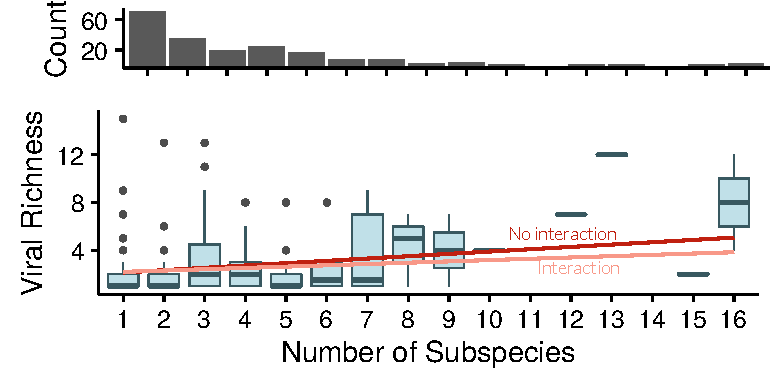
\includegraphics[width=0.8\textwidth]{figure/boxplot-1} 

}

\caption[Number of virus species against number of subspecies]{Number of virus species against number of subspecies. 
Data within a number of subspecies are plotted as boxplots with the dark bar showing the median, the box showing the interquartile range, vertical lines showing the range and outliers shown as seperate points.
Regression lines are from multivariate phylogenetic models with other independant variables set at their median value.
The models shown are thos with (pink) and without (red) an interaction between study effort and number of subspecies.
}\label{fig:boxplot}
\end{figure}


\end{knitrout}









\begin{knitrout}\footnotesize
\definecolor{shadecolor}{rgb}{0.969, 0.969, 0.969}\color{fgcolor}\begin{figure}[t]

{\centering 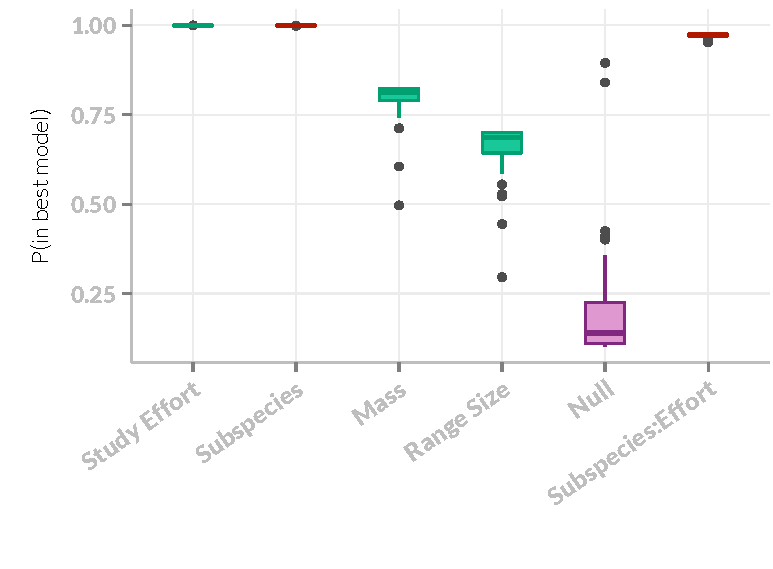
\includegraphics[width=0.8\textwidth]{figure/ITPlots-1} 

}

\caption[Akaika variable weights for number of subspecies analysis]{Akaika variable weights for number of subspecies analysis. The probability that each variable will be in the best model if the data were recollected is shown for each of the bootstrap analyses. The purple ``Null'' box is a uniform random variable used as a null. Population structure (Number of subspecies) and the interaction between subspecies and study effort, shown in red, are more likely to be in the best model than this random variable.}\label{fig:ITPlots}
\end{figure}


\end{knitrout}






\clearpage





%%%%%%%%%%%%%%%%%%%%%%%%%%%%%%%%%%%%%%%%%%%%%%%%%%%%%%%%%%%%%%%%%%%%%%%%%%%%%%%%%%%%%%%%%%%%%%%%%%%%%%%%%%%%%%%%%%%%%%%%%%%%%%%%%%%%%%%%%%%%%%%%%%%%%%%%%%%
%%%% FST ANALYSIS                                                                                                                                  %%%%%%%%
%%%%%%%%%%%%%%%%%%%%%%%%%%%%%%%%%%%%%%%%%%%%%%%%%%%%%%%%%%%%%%%%%%%%%%%%%%%%%%%%%%%%%%%%%%%%%%%%%%%%%%%%%%%%%%%%%%%%%%%%%%%%%%%%%%%%%%%%%%%%%%%%%%%%%%%%%%%






















\begin{knitrout}\footnotesize
\definecolor{shadecolor}{rgb}{0.969, 0.969, 0.969}\color{fgcolor}\begin{figure}[t]

{\centering 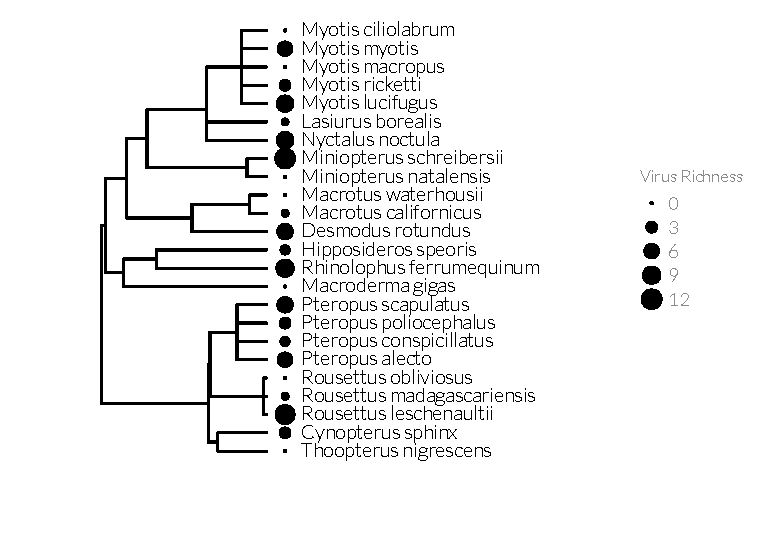
\includegraphics[width=\textwidth]{figure/fstTreePlot-1} 

}

\caption[Pruned phylogeny with dot size showing number of pathogens and colour showing family]{Pruned phylogeny with dot size showing number of pathogens and colour showing family.}\label{fig:fstTreePlot}
\end{figure}


\end{knitrout}

\begin{knitrout}\footnotesize
\definecolor{shadecolor}{rgb}{0.969, 0.969, 0.969}\color{fgcolor}

{\centering 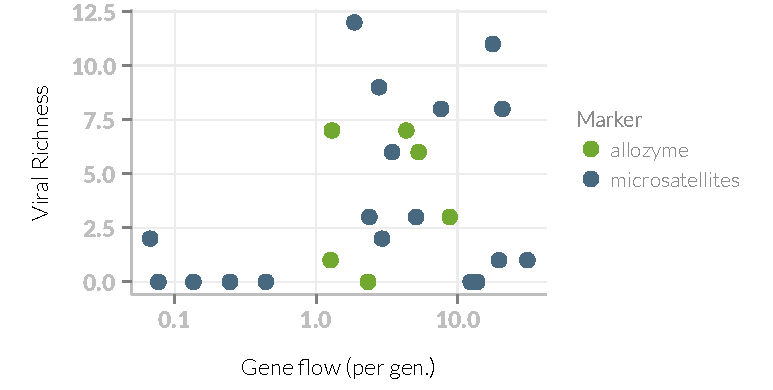
\includegraphics[width=0.8\textwidth]{figure/fstRawData-1} 

}



\end{knitrout}













\begin{knitrout}\footnotesize
\definecolor{shadecolor}{rgb}{0.969, 0.969, 0.969}\color{fgcolor}\begin{figure}[t]

{\centering 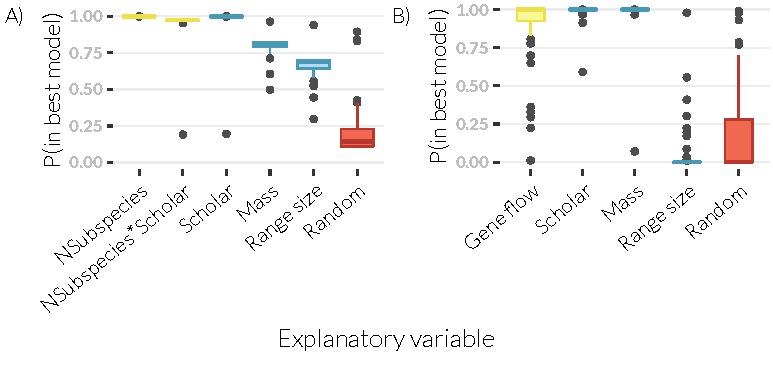
\includegraphics[width=0.8\textwidth]{figure/fstITPlots-1} 

}

\caption{Akaika variable weights for $F_{ST}$ analysis. The probability that each variable will be in the best model if the data were recollected is shown for each of the bootstrap analyses. The purple ``Null'' box is a uniform random variable used as a null. Population structure ($F_{ST}$), shown in red, is much less likely to be in the best model than this random variable.}\label{fig:fstITPlots}
\end{figure}


\end{knitrout}










$F_{ST}$ studies are conducted at a range of spatial scales, but $F_{ST}$ often increases with distance studied \cite{}.
To minimise the effects of this I only used data from studies that cover 20\% of the diameter of the species range.
This is a largely arbitrary value that could be considered to reflect a `global' estimate of $F_{ST}$ while keeping a reasonable number of datapoints available.
I calculated the diameter of the species range by finding the furthest apart points in the IUCN species range \cite{} even if the range is split into multiple polygons.
The width covered by each study was the distance between the most distant sampling sites.
When this was not explicit in the paper, the centre of the lowest level of geographic area was used.



\subsection{Statistical analysis}

Statistical analysis for both dependant variables were conducted using a information theory/model averaging approach \cite{burnham2002model} specifically following \cite{whittingham2005habitat, whittingham2006we}.
I chose a credible set of models including all combinations of independent variables.
In the analysis using the number of subspecies dependant variable I also included an interaction term between study effort and number of subspecies as I believe \emph{a priori} that this interaction may be present.
The interaction was only included in models with both study effort and number of subspecies as an individual term.

I fitted phylogenetic regressions using caper \cite{nmle} to all models.
In each case I simultaneously fitted the $\lambda$ parameter as this avoids mispecifying the model \cite{revell2010phylogenetic}.
$\kappa$ and $\delta$ were constrained to one.

As the number of data points is close to or much less than the number of variables times 40 I calculated small sample corredted AIC (AICc) for each model and then calculated Akaiki weights.
This value can be interpreted as the probability that a model would be the best model if the data were recollected.
For each variable, the sum of the Akaiki weights for models containing that variable are summed.
This value can be interpreted as the probability that the given variable is in the best model.
Following \cite{whittingham2005habitat} I included a uniformally random variable as a null variable as even unimportant variables can have Akaiki weights significantly greater than zero.
The whole analysis was run 50 times, resampling the random variable each time.
We calculated $\bar{AICc}$ by averaging AICc scores within models.
$\Delta\text{AICc}$ was calculated as $\text{min}(\bar{AICc}) - \bar{AICc}$, not the mean of the individual $\Delta\text{AICc}$ scores, to guarantee that the best model has $\Delta\text{AICc} = 0$.


Plots were created with a combination of \cite{ggplot2, palettetown, dotwhisker, ggtree}
%%%%%%%%%%%%%%%%%%%%%%%%%%%%%%%%%%%%%%%%%%%%%%%%%%%%%%%%%%%%%%%%%%%%%%%%%%%%%%%%%%%%%%%%%%%%%%%%%%%%%%%%%%%%%%%%%%%%%%%%%%%%%%%%%%%%%%%%%%%%%%%%%%%%%%%%%%%

\clearpage
\section{Results}

%%%%%%%%%%%%%%%%%%%%%%%%%%%%%%%%%%%%%%%%%%%%%%%%%%%%%%%%%%%%%%%%%%%%%%%%%%%%%%%%%%%%%%%%%%%%%%%%%%%%%%%%%%%%%%%%%%%%%%%%%%%%%%%%%%%%%%%%%%%%%%%%%%%%%%%%%%%

\subsection{Number of Subspecies}
\tmpsection{More descriptive}

After data cleaning there was data for 196 bat species in 11 families.
The number of described virus species for a bat host ranged up to 15 viruses in \emph{Carollia perspicillata}.
Figure~\ref{fig:treePlot} shows the phylogeny used and the number of viruses for each species.
The mean number of viruses across families is fairly constant with a lower range of 1.67 for Nycteridae.
The highest mean is Mormoopidae with 5 virus species per bat species, but this is based on a sample size of 3.
The Phyllostomidae have the second highest mean (n = 37) of 3.49.

The small change in mean pathogen richness across families and the lack of clear pattern in Figure~\ref{fig:treePlot} implies that viral richness is not strongly phylogenetic. 
This is corroborated by the small estimated size of $\lambda$ ($\lambda$ = , $p$ = ).
This fact implies that other factors must control pathogen richness.
It also implies that pathogens are not directly inherited down the phylogeny, although this is to be expected by the fast evolution of viruses.

Of the explanatory variables, the number of subspecies has no phylogenetic autocorrelation ($\lambda$ = , $p$ = ), study effort has weak but significant autocorrelation ($\lambda$ = , $p$ = ) and mass is strongly phylogenetic ($\lambda$ = , $p$ = ).

\tmpsection{Model results}
%See Figure \ref{fig:plotSubspeciesCoefs} for a display of estimated coefficients for the two models using number of viruses as the response variable. 
The main model with mass, study effort and number of subspecies as predictors found study effort to be highly significant ($\beta = $ NA, $p = $ \ensuremath{1.05\times 10^{-8}}). 
The number of subspecies was marginally significant ($\beta = $ NA, $p = $ 0.02). 
The effect of nonindependance due to phylogeny was very small ($\lambda = $ 0.09, $p = $ 0.02).

The interaction term between study effort and number of subspecies, when included, was significant ($\beta = $ 0.14, $p = $ \ensuremath{2.99\times 10^{-3}}).



\subsection{$F_{ST}$}











%\begin{table}[t]
%  \rowcolors{2}{gray!25}{white}
%  \begin{tabular}{lrr}
% \hline
%  Covariate & Estimate (95\% CI) & $p$ value\\
%  \hline
%  Number of subspecies & tableM[2,1] (tableM[2, 2] -- tableM[2, 3]) & tableM[2, 4]\\
%  Mass & tableM[3,1] (tableM[3, 2] -- tableM[3, 3]) & tableM[3, 4]\\
%  Study effort & tableM[4,1] (tableM[4, 2] -- tableM[4, 3]) & tableM[4, 4]\\
%  Intercept & tableM[1,1] (tableM[1, 2] -- tableM[1, 3]) & tableM[1, 4]\\
%  \end{tabular}
%\caption{Table of parameter estimates.}
%\label{t:params}
%\end{table}


\begin{table}[t]
\rowcolors{2}{gray!25}{white}
\begin{tabular}{>{\small}lrrrr}

\normalsize{Model} & $\bar{\text{AICc}}$ & $\Delta$AICc & $w_i$ & $\sum w_i$\\
\hline
log(Scholar)*NSubspecies + rand & 
896 & 0.00 &
0.14 & 0.14\\
log(Scholar)*NSubspecies & 
896 & 0.15 &
0.13 & 0.27\\
log(Scholar)*NSubspecies + rand + log(Mass) & 
896 & 0.15 &
0.13 & 0.40\\
log(Scholar)*NSubspecies  + log(Mass) & 
896 & 0.35 &
0.12 & 0.52\\
log(Scholar)*NSubspecies  + log(Mass) + log(RangeSize) & 
897 & 0.95 &
0.09 & 0.61\\
log(Scholar)*NSubspecies  + rand + log(RangeSize) & 
898 & 2.03 &
0.05 & 0.66\\
log(Scholar)*NSubspecies  + log(RangeSize) & 
898 & 2.15 &
0.05 & 0.71\\
log(Scholar) + NSubspecies & 
898 & 2.35 &
0.04 & 0.75\\
log(Scholar) + NSubspecies + log(Mass) & 
899 & 2.51 &
0.04 & 0.79
\end{tabular}
\caption{
Model selection results. 
$\bar{\text{AICc}}$ is the mean AICc score across 50 resamplings of the null random variable. 
$\Delta$AICc is the $\bar{\text{AICc}}$ score minus the lowest score. 
$w_i$ is the Akaike weight and can be interpreted as the probability that the model is the best model (of those in the plausible set).
$\sum w_i$ is the cumulative sum of the Akaike weights.}
\label{t:subsmodels}
\end{table}




%%%%%%%%%%%%%%%%%%%%%%%%%%%%%%%%%%%%%%%%%%%%%%%%%%%%%%%%%%%%%%%%%%%%%%%%%%%%%%%%%%%%%%%%%%%%%%%%%%%%%%%%%%%%%%%%%%%%%%%%%%%%%%%%%%%%%%%%%%%%%%%%%%%%%%%%%%%

\clearpage
\section{Discussion}  

%%%%%%%%%%%%%%%%%%%%%%%%%%%%%%%%%%%%%%%%%%%%%%%%%%%%%%%%%%%%%%%%%%%%%%%%%%%%%%%%%%%%%%%%%%%%%%%%%%%%%%%%%%%%%%%%%%%%%%%%%%%%%%%%%%%%%%%%%%%%%%%%%%%%%%%%%%%
















\clearpage
























\small
\printbibliography 


\end{document}
